\documentclass[]{article}

\usepackage{amsmath}
\usepackage{graphicx}
\usepackage{float}

%opening
\title{On the parametrization of additive an non-additive genetic effects}
\author{Rapha\"{e}l Scherrer}

\begin{document}

\maketitle

In our model, additive and non-additive genetic components of a given genotype-phenotype map are sampled across loci from independent distributions, whose choice of parameters influence the genetic variance in the population. The realized additive and non-additive effects can further be tuned relative to each other by means of linear scaling parameters ($\sigma_A$, $\sigma_I$, ..., see Methods). Because we exclusively use these scaling parameters to compare different genetic scenarios, this requires us to set the underlying additive and non-additive components of the genotype-phenotype map as equivalent in the amount of genetic variance they can produce. Otherwise, patterns in the observed evolutionary dynamics may arise simply because of differences in the potential of each component to generate variance in traits. Here, we present how to scale the distributions of additive and non-additive components of the genetic architecture such that the resulting potential of each to generate variance is the same.\\

To do this, we search for a correspondence between the shape and scale parameters of the locus-specific bilateral Gamma distribution of independent effect sizes $\eta$ for a given trait, respectively $k_{\eta}$ and $\theta_{\eta}$, and the shape and scale parameters of the bilateral Gamma distribution of edge-specific interaction weights $\omega$ for that same trait, respectively $k_{\omega}$ and $\theta_{\omega}$, such that the trait's genome-wide genetic variance generated by a fully additive ($\sigma_A = 1$, $\sigma_I = 0$) or fully epistatic ($\sigma_A = 0$, $\sigma_I = 1$) scenario is the same.\\

The genetic variance of the focal trait is the variance of the distribution of genetic values across the population. The genetic value of an individual is the genetically-determined component of its phenotype. Here, we assume no environmental effect for the sake of the demonstration, and we restrict ourselves to a single focal trait (the same logic applies to each evolving trait). The genetic value of an individual is the sum of the genetic values of each of its loci, where the genetic value of each locus incorporates an additive and a non-additive component, scaled by their respective scaling parameters $\sigma$ (see Methods). This means that in a fully additive scenario, the genetic value $\phi_{ik}$ of locus $i$ in individual $k$ is the locus' independent effect size multiplied by its gene expression in that individual,

\begin{equation}
	\phi_{ik} = \eta_i \, \xi_{ik}
	\label{eq:phi}
\end{equation}

Similar, in the fully epistatic scenario the genetic value $\psi_{ik}$ of locus $i$ in individual $k$ is half the contribution of all edges shared by locus $i$ with each of its partners $j$, which in turn depend on their respective interaction weights and the gene expression of both $i$ and $j$,

\begin{equation}
	\psi_{ik} = \frac{1}{2} \, \sum_j \, \omega_{ij} \, \xi_{ik} \, \xi_{jk}
	\label{eq:psi}
\end{equation}

Because all edges contribute to the trait value in Equation \ref{eq:psi}, the genetic value of the individual can be re-written, in the fully epistatic scenario, as the sum of genetic values $\psi'_{ijk}$ of each \textit{interaction} (as opposed to each \textit{locus}), where

\begin{equation}
	\psi'_{ijk} = \omega_{ij} \, \xi_{ik} \, \xi_{jk}
	\label{eq:psiprime}
\end{equation}

The locus-specific effects $\phi$ and the edge-specific effects $\psi'$ are products of bilateral Gamma-distributed variables, $\eta$ and $\omega$, with gene expression levels $\xi$, which can have, in the absence of dominance in our model, the values $-1$, $0$ or $1$. This means that, assuming that the genome of an individual is composed of a large number $N$ of loci coding for the focal trait, and that all loci have random, equally-likely genotypes (thus gene expression), in the additive scenario, approximately $1/3$ of the loci will have a zero net-effect, while for the remaining $2/3$, $\phi$ will follow the same bilateral Gamma-distribution across the genome as $\eta$. Therefore, it can be shown that $\phi$ follows a zero-inflated bilateral Gamma distribution with variance $\sigma_{\phi}^2 = 2/3 \, \sigma_{\eta}^2$.\\

Similarly, if we assume a large number of independent edges $E$ connecting random pairs of loci from a large pool of $N$ loci, and that loci have equal probability to be in either genotype, then $\xi_{ik} \, \xi_{jk}$ will be zero in $5/9$ of the cases, while for the remaining $4/9$ of the edges, $\psi'$ will follow the same bilateral Gamma distribution as $\omega$. Therefore, $\psi'$ follows a zero-inflated bilateral Gamma distribution with variance $\sigma_{\psi'}^2 = 4/9 \, \sigma_{\omega}^2$.\\

Because the genetic value of the individual is the sum of all locus-specific contributions $\phi$, in the additive case, or the sum of all edge-specific contributions $\psi'$, in the epistatic case, the central limit theorem predicts that the distribution of individual genetic values (or phenotypes, in the absence of environmental effects) in a population of randomly sampled genomes will be a normal distribution with mean zero and variance $\sigma^2$, where $\sigma^2 = N \, \sigma_{\phi}^2$ in the additive case, and $\sigma^2 = E \, \sigma_{\psi'}^2$ in the epistatic case. We can use this equality to find parameter values that yield the same population-level variance in genetic values in the additive and epistatic cases, that is, that satisfy

\begin{equation}
	N \, \sigma_{\phi}^2 = E \, \sigma_{\psi'}^2
\end{equation}

which, by substituting the variances in $\phi$ and $\psi'$ by their equivalent in terms of the underlying $\eta$ and $\omega$ distributions, corresponds to

\begin{equation}
	\frac{\sigma_{\omega}^2}{\sigma_{\eta}^2} = \frac{2}{3}\,\frac{N}{E}
	\label{eq:scaling}
\end{equation}

Here, we remind the reader that $\eta$ and $\omega$ are sampled from bilateral Gamma distributions across the genome, and are subsequently normalized by their respective sum of squares. Given an unnormalized bilateral Gamma-distributed variable $X$ with zero mean and variance $\sigma_X^2$, the corresponding normalized variable $Y = X / \sum X^2$ has a mean of zero and a variance of $1/(n^2 \, \sigma_X^2)$, where $n$ is the number of observations. Furthermore, the variance of a bilateral Gamma-distributed variable $X$ is $\sigma_X^2 = \theta^2 \, \Gamma(k+2) / \Gamma(k) $, where $\theta$ and $k$ are the shape and scale parameters of the underlying Gamma distribution, respectively. Given all of the above, Equation \ref{eq:scaling} can be written in terms of the input parameters of the model,

\begin{equation}
	\frac{\theta_{\omega}^2 \, \Gamma(k_{\omega}+2) \, \Gamma(k_{\eta})}{\theta_{\eta}^2 \, \Gamma(k_{\eta}+2) \, \Gamma(k_{\omega})} = \frac{2}{3} \, \frac{N}{E}
\end{equation}

This final equation can be used to find combinations of model parameters ensuring that the genetic variance in a large population of randomly sampled genomes at a large number of loci and with a large number of random interactions, will be the same under a fully additive and a fully epistatic genotype-phenotype map.\\

We used \textit{Mathematica} to find such suitable parameter value for the shape of the interaction weight distribution $k_{\omega}$, given $N = 1,000$, $E = 10,000$, $\theta_{\eta} = \theta_{\omega} = 1$, and $k_{\eta} = 5$. We found a value of $1$. We used these parameter values to simulate a population of 10,000 individuals and recorded their genetic values, in a fully additive and in a fully epistatic scenario, and indeed found identical distributions (Figure \ref{fig:densities}).

\begin{figure}[H]
	\centering
	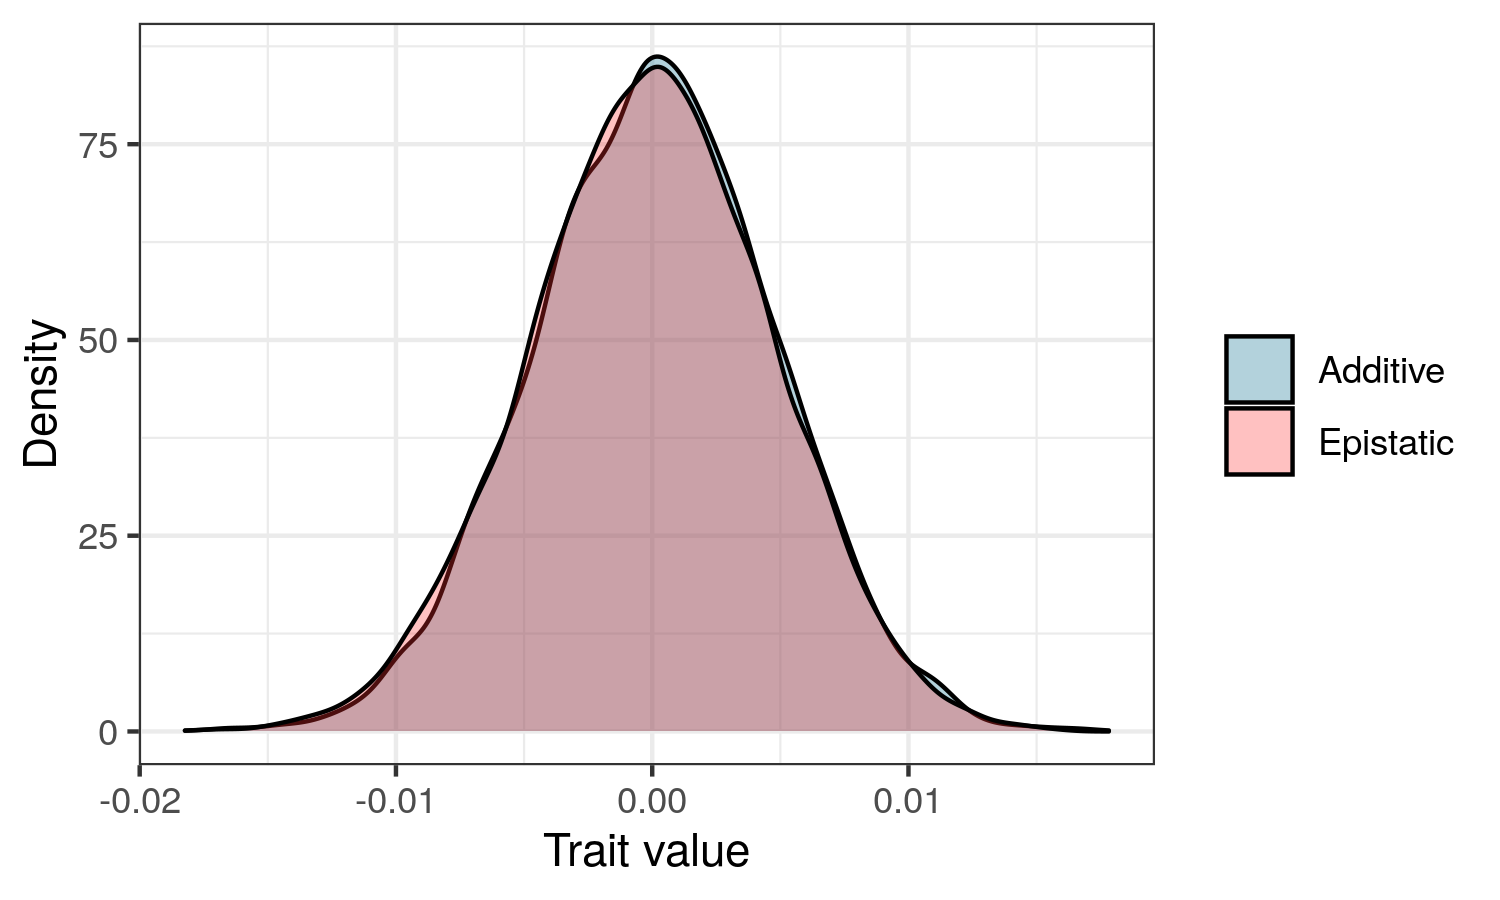
\includegraphics[width=0.8\textwidth]{gamma_param}
	\caption{Distribution of trait values in a population of 10,000 randomly generated genomes with 1,000 loci and 10,000 random edges, under fully additive or fully epistatic genetics, with the parameter values derived from our procedure.}
	\label{fig:densities}
\end{figure}

\end{document}
